% !TEX encoding = UTF-8
%Koma article
\documentclass[fontsize=12pt,paper=letter,twoside]{scrartcl}
\usepackage{float}
\usepackage{listings}
\usepackage{makecell}

%Standard Pre-amble
\usepackage[top=4cm,bottom=4cm,left=3cm,right=3cm,asymmetric]{geometry}
%\geometry{landscape}                % Activate for for rotated page geometry
%\usepackage[parfill]{parskip}    % Begin paragraphs with an empty line rather than an indent
\usepackage[table,xcdraw]{xcolor}
\usepackage{graphicx}

\usepackage{amsmath}
\usepackage{amssymb}
\usepackage{epstopdf}
\DeclareGraphicsRule{.tif}{png}{.png}{`convert #1 `dirname #1`/`basename #1 .tif`.png}
% Listings needs package courier
\usepackage{listings} % Needs 
\usepackage{courier}

\usepackage[framemethod=TikZ]{mdframed}
\usepackage{url}

\usepackage{sty/bsymb} %% Event-B symbols
\usepackage{sty/eventB} %% REQ and ENV
\usepackage{sty/calculation}

%Maths
\usepackage{amssymb,amsmath}
\def\Fl{\mathbb{F}}
\def\Rl{\mathbb{R}}
\def\Nl{\mathbb{N}}
\def\Bl{\mathbb{B}}
\def\St{\mathbb{S}}
\newcommand{\ovr}{\upharpoonright}
\newcommand{\var}[1]{\textit{#1}}
%Useful definitions
\newcommand{\mv}[1]{\textit{m\_#1}}
\newcommand{\cv}[1]{\textit{c\_#1}}
\newcommand{\degree}[1]{^{\circ}\mathrm{#1}}
%\newcommand{\comment}[1]{{\footnotesize \quad\texttt{--}\textrm{#1}}}
\newcommand{\im}[1]{i\texttt{-\!#1}}

\usepackage[headsepline]{scrpage2}
\pagestyle{scrheadings}
\ihead[]{\small EECS4312 Report1}
\ohead[]{\small \thepage}
\cfoot[]{}
\ofoot[]{}


%%%%PVS environment%%%%%%%%%%%%%%%%%%%
\lstnewenvironment{pvs}[1][]
    {\lstset{#1,captionpos=b,language=pvs,
    mathescape=true,
    basicstyle=\small\ttfamily,
    numbers=none,
    frame=single,
    % numberstyle=\tiny\color{gray},
    % backgroundcolor=\color{lightgray},
    firstnumber=auto
    }}
    {}
 %%%%%%%%%%%%%%%%%%%%%%%%%%%%%%%%
 
%%%%Verbatim environment%%%%%%%%%%%%%%%%%%%
\lstnewenvironment{code}[1][]
    {\lstset{#1,captionpos=b,
    mathescape=true,
    basicstyle=\small\ttfamily,
    numbers=none,
    frame=single,
    % numberstyle=\tiny\color{gray},
    % backgroundcolor=\color{lightgray},
    firstnumber=auto
    }}
    {}

% \newenvironment{boxed}[1]
%    {\begin{center}
%    #1\\[1ex]
%    \begin{tabular}{|p{0.9\textwidth}|}
%    \hline\\
%    }
%    { 
%    \\\\\hline
%    \end{tabular} 
%    \end{center}
%    }
 %%%%%%%%%%%%%%%%%%%%%%%%%%%%%%%%
 
 %Text in a box
\newenvironment{textbox}
    {\begin{center}
    \begin{tabular}{|p{0.9\textwidth}|}
    \hline\\
    }
    { 
    \\\\\hline
    \end{tabular} 
    \end{center}
    }

\usepackage{hyperref}

%Highlight \hl{}
\usepackage{soul}

\usepackage{enumitem}
\newlist{mylist}{itemize}{1}
\setlist[mylist]{label=\textbullet,leftmargin=1cm,nosep}

\usepackage{multirow}

% Reduce space between figure and caption
%\usepackage{caption}
%\captionsetup[table]{font=small,skip=0pt}     %% Adjust here
%or equivalently 
\usepackage[font=small,skip=4pt]{caption}
%Useful definitions
%\newcommand{\mv}[1]{\textit{m\_#1}}
%\newcommand{\cv}[1]{\textit{c\_#1}}
%\newcommand{\degree}[1]{^{\circ}\mathrm{#1}}
%\newcommand{\comment}[1]{{\footnotesize \quad\texttt{--}\textrm{#1}}}

% Set the header
\ihead[]{\small EECS4313 Assignment-2}


%%%%%%%%%%%%Enter your names here%%%%%%%%
\author{Student Name | Student Number | EECS Account
\and \textbf{Edward Vaisman | 212849857 | eddyv}
\and \textbf{Robin Bandzar | 212200531 | cse23028}
\and \textbf{Kirusanth Thiruchelvam | 212918298 | kirusant}
\and \textbf{Sadman Sakib Hasan | 212497509 | cse23152}
}
%%%%%%%%%%%%%%%%%%%%%%%%%%%%%%%%

\date{\today} % Display a given date or no date

\begin{document}
\title{EECS 4313 Assignment 2 \\Black-box and White-box Testing with JUnit}
\maketitle

\newpage

%%%%%%%%%%%%%%%%%%%%%%%%%%%%%%%
\tableofcontents


\newpage


%%%%Rest of your document goes here%%%%%%%%%%%%%%%%%%%

\section{Black Box Testing}

\subsection {Equivalence Class Testing}

\begin{itemize}
\item \textbf{Technique}: \emph{Equivalence Class Testing}
\item \textbf{Class}: \emph{net.sf.borg.common.DateUtil.java}
\item \textbf{Method}: \emph{minuteString(int mins))}
\item \textbf{Method Description}:
This method generate a human reable string for a particular numbe of minutes.It returns the string interms of hours or minutes or both hours and mintues.
\item \textbf{mins} - The argument is an integer
\item \textbf{Justification}: Equivalence class testing is suitable for this method since argument of this method is an integer which is an independent variable and the entire range of input can be partitioned while assuring disjointness and non-redundancy between each partition set. We have chosen these partition integer range based on when we use minute, minutes, hour, and hours.In order to partition the integer argument into hours and minutes,we divide the Minutes by 60 to get the range of hours and  the remainder ( minutes \% 60) to get the range of the minutes.The paritions for this method are:
 \begin{itemize}
\item \textbf{ Mins / 60 = 1 and Mins \% 60 = 0 :} To test 1 hour.
 \begin{itemize}
 \item Range of hours: [1]
 \item Range of minutes: [0]
\end{itemize}
\item \textbf{ Mins / 60 = 1 and Mins \% 60 = 1 :} To test the 1 hour with 1 minute.
 \begin{itemize}
 \item Range of hours: (1,$+\infty$)
 \item Range of minutes: [1]
\end{itemize}
\item \textbf{ Mins / 60 = 1 and Mins \% 60  $>$  1 :} To test 1 hour with minutes more than 1 minute. 
 \begin{itemize}
 \item  Range of hours: [1]
\item  Range of Minutes : (1, 59]
\end{itemize}
\item \textbf{ Mins / 60 $>$ 1 and Mins \% 60 = 0 :} To test the hours more than 1 hour.
 \begin{itemize}
 \item Range of hours: (1,$+\infty$)
 \item Range of minutes: [0]
\end{itemize}
\item \textbf{ Mins / 60 $>$ 1 and Mins \% 60 = 1 :} To test hours more than 1 hour with 1 minute. 
 \begin{itemize}
 \item Range of hours: (1,$+\infty$)
\item Range of Minutes :[1]
\end{itemize}
\item \textbf{ Mins / 60 $>$ 1 and Mins \% 60 $>$ 1 :} To test the hours more than 1 hour with minutes more than 1 minute. 
 \begin{itemize}
 \item Range of hours:  (1,$+\infty$) 
\item Range of Minutes : (1, 59]
\end{itemize}
\item \textbf{ Mins / 60 = 0 and Mins \% 60 = 0 :} To test 0 minutes.
 \begin{itemize}
 \item Range of hours: [0]
 \item Range of minutes: [0]
\end{itemize}
\item \textbf{ Mins / 60 = 0 and Mins \% 60 = 1 :} To test 1 minute.
 \begin{itemize}
 \item Range of hours: [0]
 \item Range of minutes: [1]
\end{itemize}
\item \textbf{ Mins / 60 = 0 and Mins \% 60 $>$ 1 :} To test minutes more than 1 minute and less than 60 minutes or 1 hour.
 \begin{itemize}
 \item Range of hours: [0]
 \item Range of minutes: (1,59]
\end{itemize}
\end{itemize}
The method did not specifity how negative minutes should be treated, so we omit  the negative integers as an argument for this method.For example, -75 can be converted as -1 hour and 15 minutes or 45 minutes or any other way. Therefore, this case is tested in the whitebox testing after analyzing structure of the method.
\item \textbf{Evaluation :}  The tests are shown below suitable for strong normal equivalence class testing technique since it covers the all the range of outputs for valid inputs and invalid inputs (negative integers) are not tested due to lack of specfication information regarding these values. 
 \begin{itemize}
\item \textbf{Class 1:} Mins / 60 = 1 and Mins \% 60 = 0 
\item \textbf{Class 2:}  Mins / 60 = 1 and Mins \% 60 = 1
\item \textbf{Class 3:} Mins / 60 = 1 and Mins \% 60  $>$  1
\item \textbf{Class 4:} Mins / 60 $>$ 1 and Mins \% 60 = 0
\item \textbf{Class 5:} Mins / 60 $>$ 1 and Mins \% 60 = 1
\item \textbf{Class 6:} Mins / 60 $>$ 1 and Mins \% 60 $>$ 1
\item \textbf{Class 7:} Mins / 60 = 0 and Mins \% 60 = 0
\item \textbf{Class 8:} Mins / 60 = 0 and Mins \% 60 = 1
\item \textbf{Class 9:} Mins / 60 = 0 and Mins \% 60 $>$ 1
\end{itemize}
\begin{figure}[!htb]
\begin{center}
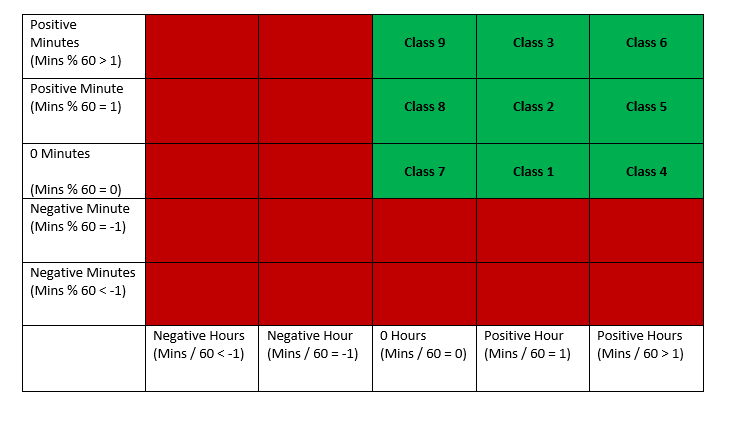
\includegraphics[width=.99\textwidth]{images/bbt/bbtmatrix.png}
\end{center}
\caption{Proving the test cases produce Strong Normal ECT}
\label{fig:bbt_matrix}
\end{figure}
In the Figure 1, The boxes colored in green represent all the valid output results and red boxes represent the invalid results which cannot be tested since the method did not specify how the negative integers should be treated. The Class 1,Class 2....Class 9 represents the partitions that we derived from how to convert the integers into readable string.


\end{itemize}

\newpage
\section{White Box Testing}

\begin{itemize}
\item The statement coverage measurements for your Assignment 2 test suite.
\item A description of the test cases that you added in this assignment to improve statement
coverage. The marker will not read your code in order to see what you tested. You have to
describe it.
\item The statement coverage measurements for your final submission. Include the screenshots of
the test running results and the screenshots of the coverage measurement. If your coverage is
not 100\%, include a discussion on why that is.
\item The Control Flow Graph you created. Indicate the segments clearly (you will probably need
to include the code for this).
\item The path coverage discussion described in section 2 above.
\item Attaching bug reports if bugs are discovered using your testing methods. You should use the
same bug report format as in Assignment 1. Do not file these bug reports to the project’s bug
report system.
\item An appendix with the specification of the methods you are testing (if there are new ones). 
\end{itemize}

\end{document}
